\chapter{Introduction}

Gyromagnetic ratios of particles in hydrogen-like bound states are an active field of experimental and theoretical research.  One series of experiments has investigated the bound $g$-factor through measurements of the spin-flip and cyclotron frequencies of hydrogen-like ions.  More recently, the same set up has been used instead to measure the electron-ion mass ratio.  This can provide an excellent determination of this ratio, but only if the theoretical bound $g$-factor ($g_b$) is known with sufficient precision.  For bound states where the particles both have spin one-half, $g_b$ is well known, but the nuclei of the ions used have a net spin zero.  In this work the leading binding and recoil corrections to $g_b$ are investigated for states of arbitrary spin.



\section{Theoretical background}


\subsection{Definition of $g$-factor}
The $g$-factor is the ratio between the magnetic moment of a particle and its angular momentum.  When considering the energy of a particle, it is the coefficient before terms that depend upon spin in the presence of a magnetic field:
 \beq
 	E \sim  g \frac{e}{2m} \v{S} \cdot \v{B}.
 \eeq
Or equivalently, it is related to the difference in energy levels between two particle of opposite spin orientation in the presence of a magnetic field:
\beq
	\Delta E =  g \frac{e}{m} \v{S} \cdot \v{B}.
\eeq


\subsection{The free $g$-factor}
The most well known $g$-factor is that of the free electron.  It may be calculated from the Lagrangian of quantum electrodynamics (QED):
\beq
	\mathcal{L} = \Psibar \left( i \partial \cdot \gamma - e A \cdot \gamma - m \right ) \Psi.
\eeq
The Dirac equation itself predicts a magnitude of $g=2$.  

When calculated in the framework of QED, there will be corrections to this ``natural'' value of $2$.  The $g$-factor being determined by the behavior of the electron in a infinitesimal magnetic field, the relevant QED calculation is the process

\vspace{1em}
\mbox{
\begin{minipage}{1in}
  \begin{center} 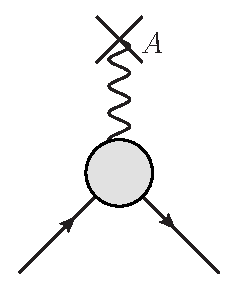
\includegraphics[scale=0.5]{eps/QED-static-field-blob} \end{center} 
\end{minipage}
=
\begin{minipage}{1in}
   \begin{center}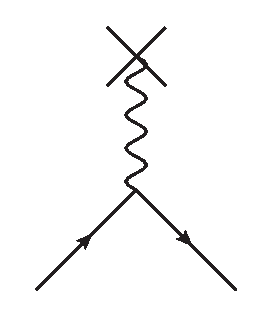
\includegraphics[scale=0.5]{eps/QEDfund}\end{center} 
\end{minipage}
+
\begin{minipage}{1in}
   \begin{center} 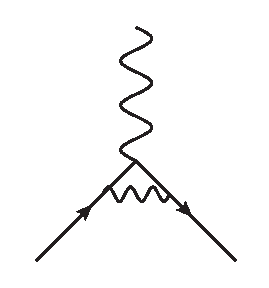
\includegraphics[scale=0.5]{eps/QEDloop1} \end{center} 
\end{minipage}
+
\begin{minipage}{1in}
   \begin{center} 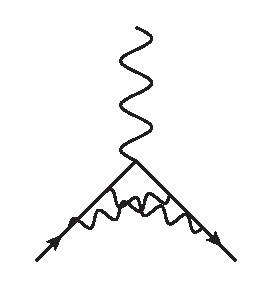
\includegraphics[scale=0.5]{eps/QEDloop2} \end{center} 
\end{minipage}
+ \hspace{2em} $\cdots$
 }
\vspace{1em} 
 
When only the fundamental vertex is calculated, the value of $2$ is obtained.  The additional loop diagrams such as illustrated above will introduce corrections to this quantity.  For an electron, these corrections will be quite small compared to the natural value of $2$. 
 
 
 
This correction to the $g$-factor is related to the anomalous magnetic moment $a_e = (g-2)/2$.  Its calculation will be a series in the coupling constant $\alpha$.   (At very high orders additional interactions will enter into the calculation, but because of the light mass of the electron compared to other particles they are highly suppressed.)  The well known first order result is
 \beq
 	a_e = \frac{\alpha}{2\pi} + \mathcal{O}( \frac{\alpha^2}{4\pi^2}).
 \eeq
The full value has been calculated to extremely high accuracy, such that the uncertainty in $g$ is 
\beq
	\frac{\Delta g}{g} \sim 10^{-13}.
\eeq

It has also been measured with a similar accuracy.  The currently accepted value \cite{Gabrielse:2006gg} is 
\beq
	g_e = \num{2.002 319 304 3622(15)},    \hspace{2em} \delta = 7.4 \times 10^{-13}.
\eeq

Because both the experimental and theoretical values are known quite precisely, these measurements of the free electron's $g$-factor provide the best determination of the constant $\alpha$.  

For the electron, the leading order term comes from the fundamental vertex, with the anomalous contribution from radiative corrections being relatively small.  In the more general case this is not true.  For example, the proton has a $g$-factor of $\sim 5.6$, where because of its composite nature the anomalous part is quite large.

It is still necessarily the case that $g$ is determined by the same process as the electron.  And this process can be parametrized by two form factors, whose value wraps up the detailed information of the high energy physics or the small scale structure of the particle. 

\subsection{Bound $g$-factors}

Even when the free $g$ factor of a particle is known, there are corrections when the particle is placed into a bound state.  Consider again the simple case of the electron, but this time it sits in a hydrogenic bound state.  It is immediately clear that the situation is much more complicated than the free case.  There are several additional scales to the problem, and so the expression for $g_b$ is no longer a series only in $\alpha$.
\begin{itemize}
  \item 	There are recoil corrections that occur when separating the internal degrees of freedom from the external motion of the whole bound system.  The related parameter is the mass ratio $m/M$	%TODO better to phrase in terms of reduced mass?
  \item 	The relativistic motion of the particle contributes binding corrections.  Because the velocity of a hydrogenic bound system is $v \sim Z\alpha$, corrections of this nature will be an expansion over $(Z\alpha)^2$.
  \item		There can be effects due to the finite size of the nucleus, although these are not considered in this work.
\end{itemize}
All of these are in addition to the radiative corrections discussed earlier; the full series will contain mixtures of all types of corrections at higher orders.

The binding corrections for the electron with $g=2$ were first calculated by Breit \cite{Breit1928}.  This can be done simply by taking the matrix element of the fundamental vertex (that responsible for the value $g=2$)  between the bound state wave functions.  This calculation of $\avg{ e\gamma \cdot A}$ gives
\beq 
	g_b =  \frac{2}{3}\left( 1 + 2 \sqrt{1 - (Z\alpha)^2}\right)  = 2 \left( 1 - \frac{(Z\alpha)^2}{3} - \frac{(Z\alpha)^4}{12} \right ).
\eeq

For the case of the proton, combined recoil and binding corrections have been known since the early 1970s.  \cite{Faustov1970422,PhysRevLett.24.39,PhysRevA.4.59}.  The bound $g$-factor of the electron was found to be
\beq
	g_b = g_e \left \{ 1 - \frac{1}{3} (Z\alpha)^2 \left[ 1 - \frac{3}{2} \frac{m}{M} + \frac{3}{2}(1+Z) \frac{m^2}{M^2} \right ]
		+ \frac{1}{4\pi} \alpha (Z\alpha)^2 \left[ 1 - \frac{5}{3} \frac{m}{M} + \frac{6+Z}{3} \frac{m^2}{M^2} \right ] \right \}.
\eeq

%TODO add g=2 + a_e result for spin half?
A more general result, valid for arbitrary spin, is of not only abstract interest.  As discussed later, there are very sensitive experiments which involve nuclei with spin other than one-half.  A result valid for such systems is necessary to extract useful information from the experiments.
	

There are already two extant approaches to this problem.  A method based on the Bargmann-Michel-Telegdi (BMT) equation was utilised by Eides and Grotch \cite{Eides:1997sq}.  Leading relativistic and recoil corrections are calculated, with the result that they are in fact independent of spin.  This follows from the form of the BMT equation, which itself carries no dependence on spin.  The leading order correction to $g$ for a hydrogenic atom was found to be
\beq
	\Delta g_{EG} = (1 + Z)(Z\alpha)^2 \left( \frac{m_e}{M} \right )^2.
\eeq 

In \cite{doi:10.1139/p02-112} Faustov and Martynenko used a quasipotential framework to calculate $g_b$.  Here the result was found to depend upon the spin of the particle.  For a spin-half particle there is agreement between this and the above approach, but clearly in general there is disagreement.   For a hydrogenic atom with a spin-0 nucleus, the result was
\beq
	\Delta g_{FM} = \frac{Z}{3} (Z\alpha)^2 \left( \frac{m_e}{M} \right )^2.
\eeq
To give a concrete idea of the discrepancy produced by the methods, here are the numerical results pertinent to the previously mentioned experiments:  
\begin{center}
\begin{tabular}{r c c}
 					&	$\hC$						&	 $\hO$	\\	\hline
 $\Delta g_{EG}$		&	$ 0.28 \times 10^{-10}$ 	&	$ 0.36 \times 10^{-10}$	\\
 $\Delta g_{GM}$		&	$ 0.80 \times 10^{-11}$		&	$ 0.11 \times 10^{-10}$	\\
 Discrepancy			&	$ 0.2 \times 10^{-10}$		&	$ 0.25\times 10^{-10}$	\\
\end{tabular}
\end{center}

Such discrepancies directly effect the experiments previously discussed, so a resolution to the situation is of practical concern.





\section{Experimental background}
A first set of experiments measuring the bound state $g$-factor were done in the sixties and seventies.  Systems investigated included hydrogen \cite{PhysRev.139.A19,PhysRevLett.39.602,PhysRevA.5.83}, deuterium \cite{PhysRevLett.28.1159}, tritium \cite{PhysRevA.9.1543}, and helium \cite{PhysRevLett.45.250}.  Such experiments allowed comparison to the theoretical value of $g_b$.

Starting in the late nineties, more precise experimental results were obtained for hydrogen-like lead \cite{PhysRevLett.81.4824}, bismuth \cite{GSI:1999}, and carbon \cite{PhysRevLett.85.5308}.  Since then steady progress has been made; the best current results come from hydrogen-like carbon \cite{PhysRevLett.85.5308,springerlink:10.1140/epjd/e2003-00012-2} and oxygen \cite{Verdu:November2002:1208-6045:1233,PhysRevLett.92.093002}.


These experiments, which can be used to measure the bound $g$-factor, proceed roughly as follows.  A system is placed in a weak magnetic field $B$, and the spin flip frequency $\omega_L$, corresponding to transitions between Zeeman levels, is measured.   $\omega_L$ is proportional to the bound factor $g_b$:
\beq
	\omega_L = g_b \frac{e}{2m_e} B.
\eeq

The cyclotron frequency $\omega_C$ is
\beq
	\omega_C = (Z-1) \frac{eB}{M}.
\eeq

So the ratio of these frequencies gives
\beq
	\frac{\omega_L}{\omega_C} = \frac{f_L}{f_C} = 
	g_b \frac{e}{2(Z-1)} \frac{M}{m_e}.
\eeq
This ratio doesn't depend on $B$, but does depend upon $g_b$ and the ratio of the electron mass ratio $m_e/M$.  Earlier experiments used this to measure $g_b$.  However, if the theoretical value fore $g_b$ is known precisely enough, the experiment can instead be used to provide a measurement of the mass ratio.  
\beq
	\frac{m}{M} = \frac{g_b}{2(Z-1)} \frac{\omega_C}{\omega_L}.
\eeq


The best current measurements for these systems are discussed in \cite{2006IJMSp.251..152W}.  For $\hC$ ($Z=6$) the value is
\beq
	 \frac{f_L}{f_C} = \num{4376.2104989(23)},	\hspace{3em} 	\delta= 5.2 \times 10^{-10}.
\eeq

And for $\hO$ ($Z=8$)
\beq
		 \frac{f_L}{f_C} = \num{4 164.376 1837 (32)}, \hspace{3em} \delta= 7.6 \times 10^{-10}.
\eeq

With such precision, these experiments became the best source for values of the electron mass in atomic units, but only if the theoretical value of the $g$-factor is also precisely known.  The current measurements above have an uncertainty of $ \sim 10^{-10}$, but in the future this is expected to improve to $\delta \sim 10^{-12}$. \cite{Jentschura2006102,Quint:2008}.  To fully exploit such sensitivity requires $g_b$ to be known with matching precision.  



\section{Calculation of binding and recoil corrections to $g_b$ for arbitrary spin}
The goal is to calculate the leading binding and recoil corrections to the bound state $g$-factor for loosely bound systems of arbitrary spin.  The binding corrections will be of order $v^2=(Z\alpha)^2$ relative to the first order terms. They are relativistic in nature, but the loosely bound systems are nonrelativistic.  So the general idea is to derive a nonrelativistic Hamiltonian or Lagrangian which incorporates corrections from a relativistic theory, and then use that to calculate the binding and recoil corrections to the bound $g$-factor.

First a nonrelativistic Lagrangian will be derived for particles of spin one-half and spin one in the known framework of quantum electrodynamics.  There are two ways to go.  A technique based on the Foldy-Wouthyusen transformation will be used first, to find a nonrelativistic Hamiltonian.  Then the results will be replicated with a diagrammatic approach that develops the most general form of an effective nonrelativistic Lagrangian, and fixes the particular coefficients of terms by comparing scattering amplitudes.

Then the theory of arbitrary spin particles will be considered.  A form of nonrelativistic Lagrangian valid for any spin will be developed.  By using the symmetries necessary for a relativistic theory, the same amplitude calculated diagrammatically in the spin one-half and spin one cases is found.  This is used to find the coefficients for the general spin effective Lagrangian.

Using this Lagrangian, the bound state problem is approached.  The effective interaction potential is derived.  Separation of the center of mass motion is achieved, and finally the bound state $g$-factor is calculated.




